\documentclass[25pt, a0paper, landscape]{tikzposter}

% ============================================================
% Packages
% ============================================================
\usepackage[T1]{fontenc}
\usepackage{lmodern}
\usepackage{graphicx}
\usepackage{enumitem}

% Remove tikzposter watermark
\tikzposterlatexaffectionproofoff

% Define VeryHuge if not available in this tikzposter version
\makeatletter
\@ifundefined{VeryHuge}{%
  \newcommand{\VeryHuge}{\fontsize{80}{96}\selectfont}%
}{}
\makeatother

% ============================================================
% Color Theme — RoCam Red / Black
% ============================================================
\definecolorstyle{RoCamStyle}{
  \definecolor{colorOne}{RGB}{30, 30, 30}       % dark (headers)
  \definecolor{colorTwo}{RGB}{220, 38, 38}      % RoCam red
  \definecolor{colorThree}{RGB}{245, 245, 245}  % light gray
}{
  \colorlet{backgroundcolor}{white}
  \colorlet{framecolor}{white}
  % title bar
  \colorlet{titlefgcolor}{white}
  \colorlet{titlebgcolor}{colorOne}
  % blocks
  \colorlet{blocktitlebgcolor}{colorOne}
  \colorlet{blocktitlefgcolor}{white}
  \colorlet{blockbodybgcolor}{white}
  \colorlet{blockbodyfgcolor}{black}
  % inner blocks
  \colorlet{innerblocktitlebgcolor}{colorTwo}
  \colorlet{innerblocktitlefgcolor}{white}
  \colorlet{innerblockbodybgcolor}{colorThree}
  \colorlet{innerblockbodyfgcolor}{black}
}

\usetheme{Default}
\usecolorstyle{RoCamStyle}
\useblockstyle{Default}
\usetitlestyle{Filled}
\makeatletter
\setlength{\TP@blockverticalspace}{8mm}
\makeatother

% Consistent image card for poster visuals
\newcommand{\posterimg}[3][]{%
  \begin{minipage}[t]{\linewidth}
    \centering
    \setlength{\fboxsep}{0pt}%
    \fcolorbox{colorOne!40}{white}{\includegraphics[#1]{#2}}\\[0.12em]
    {\footnotesize\bfseries #3}
  \end{minipage}%
}

% ============================================================
% Title — three-part header: McMaster | Logo+Title | Department
% ============================================================
\title{\mbox{}}
\author{}
\institute{}

\makeatletter
\settitle{
  \parbox{\linewidth}{%
    \color{titlefgcolor}%
    \begin{minipage}[c]{0.20\linewidth}
      {\Large\bfseries McMaster University\\[0.15em] Engineering}
    \end{minipage}%
    \hfill
    \begin{minipage}[c]{0.52\linewidth}
      \centering
      \includegraphics[height=7cm]{../assets/logo/red.png}\\[0.3em]
      {\huge High Performance Vision-Guided Rocket Tracker}
    \end{minipage}%
    \hfill
    \begin{minipage}[c]{0.22\linewidth}
      \raggedleft
      {\LARGE\bfseries Capstone Project}\\[0.3em]
      {\Large Department of\\Computing and Software\\[0.2em]
       Mechatronics \&\\Software Engineering}
    \end{minipage}%
  }%
}
\makeatother

% ============================================================
\begin{document}
\maketitle

\begin{columns}

% ============================================================
%  LEFT COLUMN
% ============================================================
\column{0.48}

% --- Motivation ---
\block{Motivation}{
  Capturing smooth, stable footage of model rockets is a major challenge.
  These vehicles accelerate to hundreds of meters per second within fractions
  of a second, making manual camera tracking nearly impossible. Existing
  commercial tracking solutions are prohibitively expensive and not designed
  for amateur rocketry.

  \vspace{0.25em}

  RoCam addresses this gap with an \textbf{autonomous, vision-guided camera
  tracking system} that locks onto and follows model rockets in real time.
  The system delivers smooth \textbf{1080p video at 60\,fps}, capturing
  critical flight events such as motor ignition, staging, and parachute
  deployment.

  \vspace{0.25em}

  Designed for small-scale launches ($<$200\,m apogee), the platform is
  \textbf{scalable to high-powered rockets} (3\,km+ apogee) for
  organizations such as the McMaster Rocketry Team.

  \vspace{0.5em}

  \centering
  \posterimg[
    width=0.96\linewidth,
    keepaspectratio
  ]{libs/section_1.png}{RoCam Launch and Tracking Operations}
}

% --- System Architecture ---
\block{System Architecture}{
  % --- Left Side: Diagram ---
  \begin{minipage}[c]{0.58\linewidth}
    \centering
    \posterimg[
      width=\linewidth,
      clip
    ]{../img/pipeline.png}{Real-Time Vision and Control Pipeline}
  \end{minipage}% <--- Crucial % to prevent Overfull \hbox
  \hfill
  % --- Right Side: Text ---
  \begin{minipage}[c]{0.40\linewidth}
    \small
    \noindent\textbf{Edge Compute \& Hardware.} The implemented architecture follows a distributed multi-process edge-compute design on an NVIDIA Jetson. To ensure high reliability, CPU/GPU-heavy perception workloads are isolated from control and operator services via Inter-Process Communication (IPC). This strict fault isolation preserves deterministic command flow and API stability even if the vision pipeline encounters transient errors during launch-dynamic conditions.

    \vspace{0.6em}
    \noindent\textbf{Vision Pipeline.} Image acquisition utilizes a GStreamer capture graph configured for 1920$\times$1080 at 60\,fps, feeding NVIDIA DeepStream for GPU-accelerated preprocessing. Detection relies on a YOLO network optimized with TensorRT, yielding low-latency normalized bounding boxes. A decoupled Live Video process parallelizes OSD telemetry overlay and HDMI output to guarantee continuous situational awareness without blocking inference.

    \vspace{0.6em}
    \noindent\textbf{Kinematic Control.} The tracking module calculates image-plane target error (targeting frame center $cx=0.5, cy=0.5$) to generate proportional 2-axis gimbal actuation commands. These commands pass through a validated, state-gated pathway—enforcing rate limits and safety bounds—before transmission to an STM32 microcontroller via UART, ensuring deterministic, closed-loop responsiveness throughout boost and coast regimes.

    \vspace{0.6em}
    \noindent\textbf{Backend \& State Management.} System orchestration is governed by a centralized State Machine (Disarmed, Armed, Tracking, Recording) that prevents invalid mode combinations and enforces hardware safety. A Flask-based API Gateway exposes a REST interface for offline-first LAN operation, managing mode transitions, asynchronous recording/transcoding workflows, and streaming SSE telemetry for live state and control-stream observability.
  \end{minipage}
}

% ============================================================
%  RIGHT COLUMN
% ============================================================
\column{0.48}

% --- Key Features ---
\block{Key Features}{
  \begin{minipage}[t]{0.57\linewidth}
    \centering
    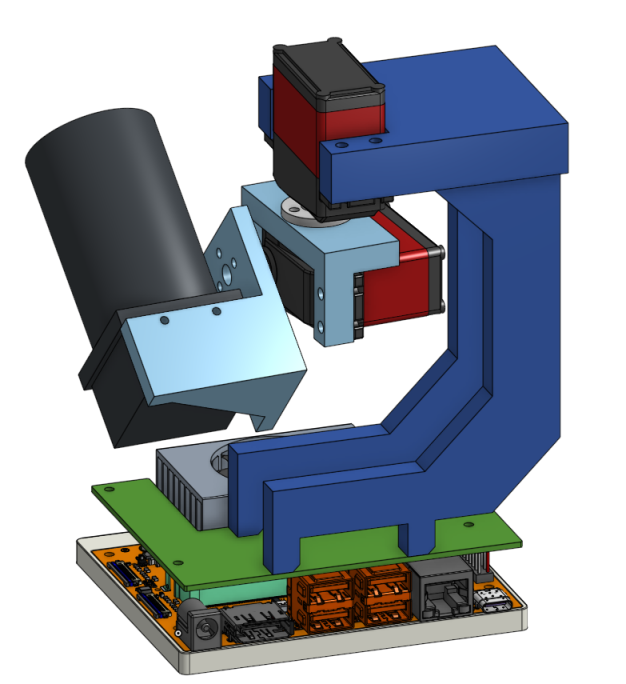
\includegraphics[width=\linewidth]{libs/prototype.png}\\[0.3em]
    {\normalsize\bfseries Web-Based Operator Interface}
  \end{minipage}%
  \hfill
  \begin{minipage}[t]{0.38\linewidth}
    \centering
    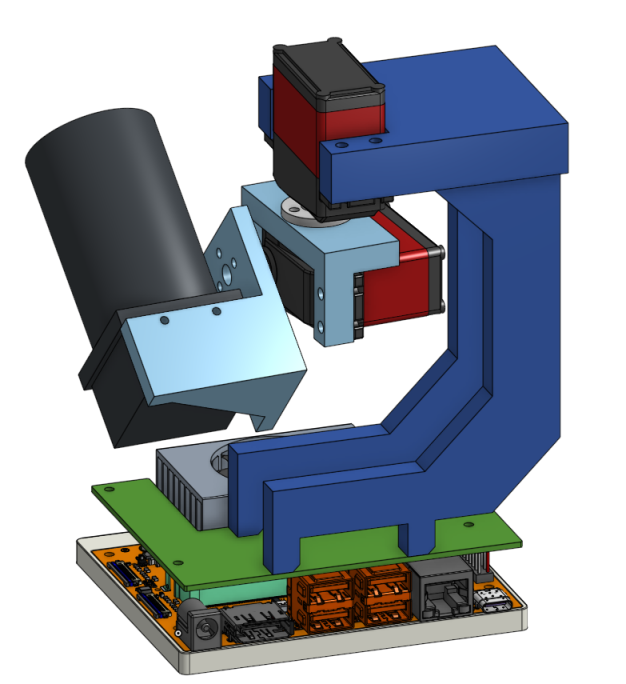
\includegraphics[width=0.85\linewidth]{libs/prototype.png}\\[0.3em]
    {\normalsize\bfseries Two-Axis Gimbal Prototype}
  \end{minipage}

  \vspace{0.8em}

  \begin{itemize}[leftmargin=1.2em, itemsep=0.4em]
    \item \textbf{Real-Time Gimbal Control} -- Two-axis servo gimbal with
          closed-loop proportional control for smooth, accurate tracking.
    \item \textbf{YOLO Computer Vision} -- GPU-accelerated object detection
          via NVIDIA DeepStream and TensorRT, maintaining lock through
          partial occlusion.
    \item \textbf{Web Application} -- Live 1080p video preview, manual
          override controls, video recording with playback and download.
    \item \textbf{Digital Zoom \& Stabilization} -- Software-based zoom
          and frame stabilization for clear close-up footage of rocket events.
  \end{itemize}
}

% --- Tools & Technologies ---
\block{Tools \& Technologies}{
  \centering
  
\includegraphics[width=0.88\linewidth, keepaspectratio]{libs/tools.png}
}

% --- Team Section ---
\block{Our Team}{
  \begin{minipage}[t]{0.28\linewidth}
    
    % --- COLOR CHANGE ADDED HERE ---
    \colorlet{innerblocktitlebgcolor}{green!40!black} % Mixes green with 60% black for a deep forest green
    \colorlet{innerblocktitlefgcolor}{white}          % Ensures the header text stays white
% -------------------------------
    % -------------------------------

    \innerblock{Development Team}{
      \small\sffamily 
      \begin{minipage}[t][7.2cm][c]{\linewidth} 
        \centering
        
\includegraphics[width=0.85\linewidth, height=2.8cm, keepaspectratio]{libs/team_rocam.png}\\[1em]
        Zifan Si\\[0.2em]
        Jianqing Liu\\[0.2em]
        Mike Chen\\[0.2em]
        Xiaotian Lou
      \end{minipage}
    }
  \end{minipage}%
  \hfill
  \begin{minipage}[t]{0.28\linewidth}
    \innerblock{Launch Team}{
      \small\sffamily
      \begin{minipage}[t][7.2cm][c]{\linewidth}
        \centering
        
\includegraphics[width=0.85\linewidth, height=3.0cm, keepaspectratio]{libs/team_rocketry.png}\\[1em]
        McMaster Rocketry Team
      \end{minipage}
    }
  \end{minipage}%
  \hfill
  \begin{minipage}[t]{0.28\linewidth}
    
    % --- COLOR CHANGE ADDED HERE ---
    \colorlet{innerblocktitlebgcolor}{blue!80!black} % Changes the header background to blue
    \colorlet{innerblocktitlefgcolor}{white}         % Ensures the header text stays white
    % -------------------------------

    \innerblock{Advisory Team}{
      \small\sffamily
      \begin{minipage}[t][7.2cm][c]{\linewidth}
        \centering
        Dr.\ Shahin Sirouspour\\[0.2em]
        Dr.\ Spencer Smith\\[0.2em]
        Tanya Djavaherpour\\[1em]
        
\includegraphics[width=0.85\linewidth, height=2.8cm, keepaspectratio]{libs/team_cas.png}
      \end{minipage}
    }
  \end{minipage}
}
\end{columns}
\end{document}
